\documentclass{standalone}
\usepackage{tikz}
\usepackage{tabularx}
\usepackage{colortbl}
\usepackage{booktabs}

\begin{document}
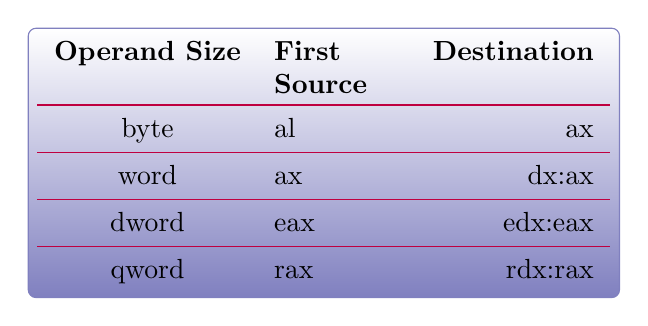
\begin{tikzpicture}[tab_style/.style={
		draw=blue!50!black!50,
		top color=white,
		bottom color=blue!50!black!50,
		rounded corners=1mm
	}]

\node[tab_style](tbl) {
\begin{tabularx}{.6\textwidth}{cXrcc}
\arrayrulecolor{purple}
\textbf{Operand Size} & \textbf{First Source} & \textbf{Destination} \\
\toprule
byte & al & ax \\
\midrule
word & ax & dx:ax \\
\midrule
dword & eax & edx:eax \\
\midrule
qword & rax & rdx:rax
\end{tabularx}
};

\end{tikzpicture}
\end{document}
